\documentclass{article}
\usepackage[T1]{fontenc}
\usepackage{lmodern}
\usepackage{graphicx}
\usepackage{amsmath,amssymb}
\usepackage[a4paper,margin=2cm]{geometry}
\usepackage[absolute,overlay]{textpos}
\setlength{\TPHorizModule}{1mm}
\setlength{\TPVertModule}{1mm}
\usepackage[indonesian]{babel}
\usepackage{hyperref}
\setlength{\emergencystretch}{2em}
% unit: Halaman 11

\begin{document}

% === Halaman 11 (llm) ===

\vspace{222.75mm}

\begin{itemize}
    \item Kakas online untuk menghitung frekuensi kemunculan huruf, bigram, trigram dsb: \url{https://www.cryptool.org/en/cto/n-gram-analysis}
\end{itemize}
\vspace{10mm}

% deskripsi: Screenshot halaman web CrypTool-Online untuk analisis N-gram yang menunjukkan input teks ciphertext dan pengaturan panjang tabel serta n-gram.
% bbox normalisasi: [0.1400, 0.1800, 0.8900, 0.9300]
\begin{textblock*}{157.50mm}(29.40mm,53.46mm)
\noindent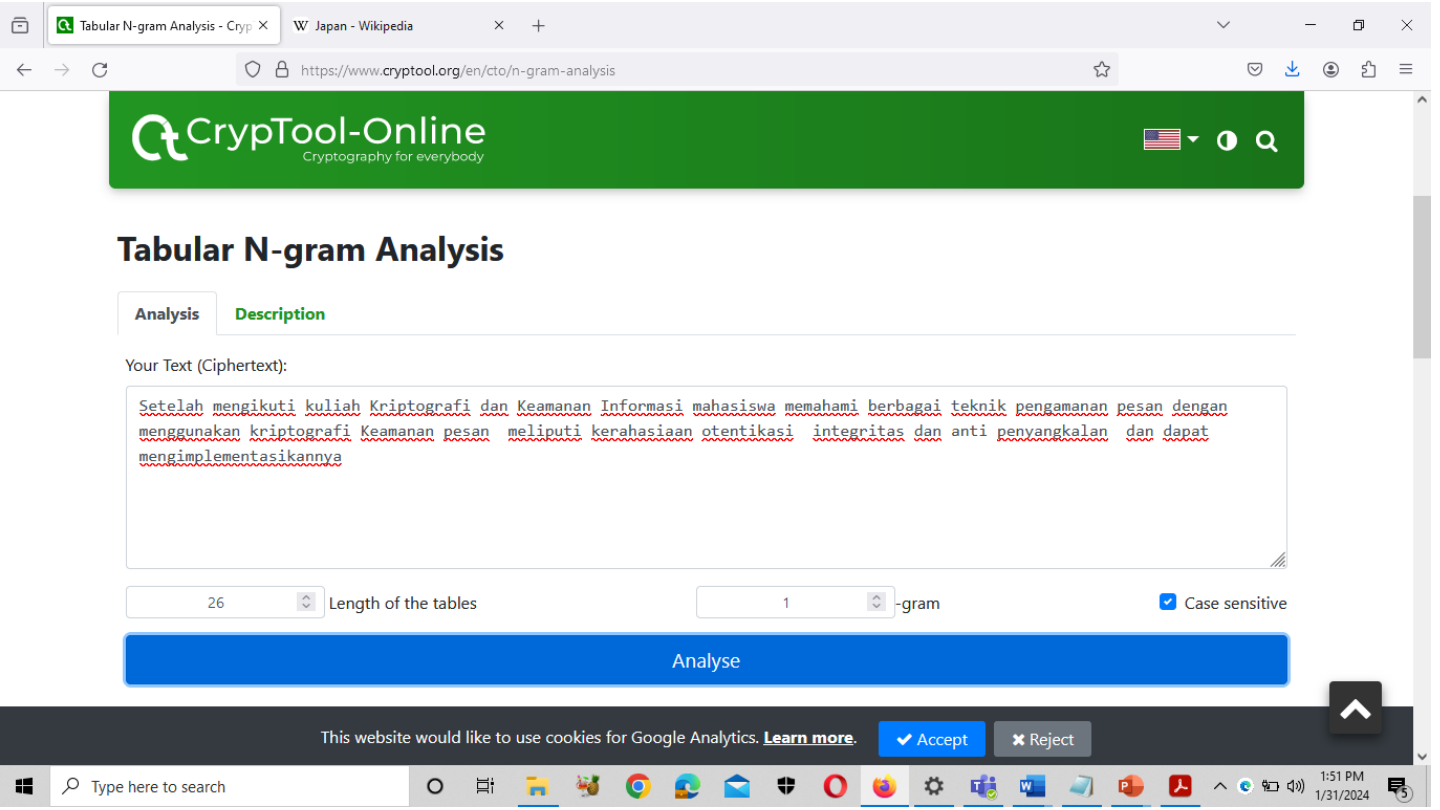
\includegraphics[width=157.50mm,height=222.75mm]{../../images/llm/page_011_img_01.png}%
\end{textblock*}

\end{document}
